\chapter{Results}
\label{result}

In this chapter, we report the results from all of our experiments and additional observation from the neural network's behavior.
It was reported that choosing a stopping criterion for NMT models is tricky \citep{TrainingTipsfortheTransformerModel} depending on many aspects.
We opted to stop training our models after 500000 steps, at which the \transformerbase was observed to show the sign of convergence.

\section{Enriching Encoder}
\label{result-enriching}

% \cref{tab:res-enriching} reports the results for our effort to enrich the \transformer model.

\subsection{Tree Distance and Traversal}

For the tree distance and tree traversal, it is shown that replacing the positional encoding or relative position with our proposed tree-related encodings does not help the translation.
All of the proposed methods are worse than the baselines.

As listed in \cref{tab:res-enriching}, on the test set, \transformerbase and \transformerrel achieved 36.66 and 37.02 BLEU, respectively, whereas \TreeTraversal, \TreeDistance max 5 and max 20 only got 35.80, 33.13 and 35.50 BLEU, in that order. However, when the tree distance was combined with the positional encoding (\transformerbase) or the relative position (\transformerrel), it yielded better results than both baselines (37.49 and 37.55 vs. 36.66 and 37.02). This is also applied to the case of tree traversal (37.80 vs. 37.02).

\begin{table}[t]
    \begin{center}
    \begin{tabular}{lcc}
        \textbf{Model}        	                            & \textbf{Dev}	& \textbf{Test}	\\
        \hline
        \transformerbase (base)    					        & 37.28 & 36.66 \\
        \transformerrel	(relative)				            & 37.23 & 37.02$^{\dag}$ \\
        \hline
        \TreeDistance, max 5				                & 35.47 & 33.13 \\
        \TreeDistance, max 20				                & 34.45 & 35.50 \\
        \TreeTraversal					                    & 35.21 & 35.80 \\
        (base) + \TreeDistance, max 5					    & 37.67 & 37.49$^{\ddag\blacktriangledown}$ \\
        % (base) + tree distance, max 20					    &  &  \\
        % (base) + tree traversal					        &  &  \\
        (relative) + \TreeDistance, max 20			        & 37.15 & 37.55$^{\ddag\blacktriangledown}$ \\
        (relative) + \TreeTraversal				            & 38.22 & \textbf{37.80}$^{\ddag\blacktriangledown}$ \\
        \hline
        (base) + \SpecPOS						& 36.97 & 36.65 \\
        (relative) + \SpecPOS			& 37.81 & 36.93$^{\dag}$ \\
        (base) + \SpecDep		& 37.53 &  37.72$^{\ddag\blacktriangledown}$ \\
        (relative) + \SpecDep		& 37.66 & \textbf{37.97}$^{\ddag\blacktriangledown}$  \\
    \end{tabular}
    \end{center}
    \caption{Enriching encoder results on \cs2en. Statistical significances are marked as $\dag p < 0.05$ and $\ddag p < 0.01$ when compared to the \transformerbase and $\triangledown/\blacktriangledown$ when compared to the \transformerrel.}
    \label{tab:res-enriching}
\end{table}

\subsection{Specialized Attention Head}

Also in \cref{tab:res-enriching}, for our second approach in the direction of enriching the encoder, the \SpecPOS model, whose one head in layer 0 was chosen to be dedicated as a specialized POS head, could not surpass the baselines (36.65 vs 36.66, 36.93 vs 37.02).

On the other hand, guiding this specialized attention head with dependency label embedding brought $+1.06$ BLEU over the \transformerbase (37.72 vs 36.66).
In addition, \SpecDep when combining with \transformerrel also achieved $+0.95$ BLEU over the \transformerrel (37.97 vs 37.02).

\section{Interpreting Self-Attention as Parse}
\label{result-promote}

\subsection{Diagonal Parsing}
\label{result-promote-diagonal}

Before discussing the result of the parsing tasks (diagonal parsing and dependency parsing), we would like to note that a multi-task model usually requires much longer time to train compared to the single task model, e.g. twice of the training time.
However, all of our multi-task models discussed in this section and the following sections were also trained for only 500000 steps.
The comparison of training time will be reported in \cref{result-speed}.

\cref{tab:res-translate-monoparse} reveals the result of our joint model which is capable of translating and parsing the source sentence to the diagonal matrix.
The diagonal parsing precision is, as expected, very high, from 99.95\% to 99.99\% on the test set.
This joint model also outperformed the baseline in translation task with all of its variants (BLEU scores vary from 37.47 to 38.14, against 36.66).

Moreover, these results form an observable pattern, in which the best result comes from the model which syntax (diagonal matrix) is demanded from the head on layer 0, then the BLEU scores decrease when it come to deeper layers.
We believe a possible explanation for this pattern is because the diagonal matrix represents the relation between the preceding token and the current token.
This is a very simple sentence structure and serves as an additional positional information to the absolute position embeddings.
Therefore, the sooner the model is forced to recognize this information (via training the parsing task), the better it can learn to do translation.

\begin{table}[t]
\centering
\vspace{2ex}
  \begin{tabular}{lcc|cc}
    &  \multicolumn{2}{c}{\textbf{BLEU}} & \multicolumn{2}{|c}{\textbf{Precision}} \\
    & \textbf{Dev} & \textbf{Test} & \textbf{Dev} & \textbf{Test} \\
    \hline
    \transformerbase & 37.28 & 36.66 & -- & -- \\
    \hline
    Syntax demanded from head on layer 0 & 38.68 & \textbf{38.14} & 99.97 & 99.96 \\
    Syntax demanded from head on layer 1 & 39.11 & 38.06 & 99.99 & \textbf{99.99} \\
    Syntax demanded from head on layer 2 & 37.85 & 37.85 & 99.98 & 99.98 \\
    Syntax demanded from head on layer 3 & 37.93 & 37.70 & 99.97 & 99.98 \\
    Syntax demanded from head on layer 4 & 37.68 & 37.47 & 99.98 & 99.96 \\
    Syntax demanded from head on layer 5 & 37.53 & 37.54 & 99.96 & 99.95 \\
  \end{tabular}
  \caption{\DiagonalParse's results in translation (BLEU) and diagonal parsing (precision) on \cs2en. All test BLEU scores are statistical significant with $p<0.01$ when compared to the \transformerbase.}
  \label{tab:res-translate-monoparse}
\end{table}

\subsection{Dependency Parsing}
\label{result-promote-dependency}

Analogous to \cref{tab:res-translate-monoparse}, \cref{tab:res-translate-depparse} presents the results of our joint dependency parsing and translation model.

Let us recall the discussion in \cref{multitask-dep-parsing} that the choice of the head from one layer which will serve as the dependency parse is arbitrary.
However, selecting which layer matters.
In the \transformer's encoder of our experiments, there are six multi-head attention layers.
\cref{tab:res-translate-depparse} shows the result of both tasks when different layers in the encoder were chosen to dedicate one of its self-attention heads to be the dependency matrix.

It is apparent from \cref{tab:res-translate-depparse} that layer 0 (the first layer) was a too shallow layer to demand the syntax from.
Demanding dependency syntax from this layer yielded undesirable results in both translation and parsing task.
The BLEU score of 36.60 is no improvement over the baseline (36.66), while the UAS is at least 8\% lower than other variants of the same model.
We believe this result was caused by the fact that the self-attention mechanism at this layer purely compared between input word embeddings, which perhaps might tend to concern more about lexical meaning than syntax.
Therefore, it could not capture the complex dependency syntax, which is not as simple as the diagonal syntax mentioned in the previous section.
On the other hand, layer 1 performed well on the parsing task (90.78\%), and brought the best improvement to the translation task (38.01).
The translation performance seems to be decreasing when it comes to the deeper layers as well (38.01 - 37.87 - 37.67 - 37.60), which phenomenon we have observed in the diagonal parsing.
The reason, from our point of view, is also similar.
The dependency syntax should be introduced to the model early enough in order to encourage better attention, but not too early.

The performance on the dependency parsing task is shown to behave in the opposite direction.
The UAS values in \cref{tab:res-translate-depparse} are increasing from the shallower to the deeper layer (82.85 - 90.78 - 91.18 - 91.43 - 91.56).
The highest UAS was achieved when the syntax is demanded from layer 4, while the model was still able to maintain good translation performance.
This pattern could suggest that when reaching to the deeper layers, the encoder has already learned a good representation for each tokens.
By good, we mean that the information from other tokens and the relation between those and the current token have been well synthesized by the shallower layers.
Therefore, at these deeper layers, the model can easily infer the dependency syntax.

\begin{table}[t]
\centering
\vspace{2ex}
  \begin{tabular}{lcc|cc}
    &  \multicolumn{2}{c}{\textbf{BLEU}} & \multicolumn{2}{|c}{\textbf{UAS}} \\
    & \textbf{Dev} & \textbf{Test} & \textbf{Dev} & \textbf{Test} \\
    \hline
    \transformerbase & 37.28 & 36.66 & -- & -- \\
    \hline
    Syntax demanded from head on layer 0 & 36.95 & 36.60 & 81.39 & 82.85 \\
    Syntax demanded from head on layer 1 & 38.51 & \textbf{38.01} & 90.17 & 90.78 \\
    Syntax demanded from head on layer 2 & 38.50 & 37.87 & 91.31 & 91.18 \\
    Syntax demanded from head on layer 3 & 38.37 & 37.67 & 91.43 & 91.43 \\
    Syntax demanded from head on layer 4 & 37.86 & 37.60 & 91.65 & \textbf{91.56} \\
    Syntax demanded from head on layer 5 & 37.63 & 37.67 & 91.44 & 91.46 \\
  \end{tabular}
  \caption{\DepParse's results in translation (BLEU) and dependency parsing (UAS) on automatically annotated data (\cs2en). All test BLEU scores, except on layer 0, are statistical significant with $p<0.01$ when being compared to the \transformerbase.}
  \label{tab:res-translate-depparse}
\end{table}

It is important to remind the reader that the parsing results reported up to this moment were computed against the auto-generated treebanks come with the parallel corpus.
Hence, to have a better sense of how our models perform compared to the gold-annotated dataset, we tested our models with the PDT test set for Czech.
The referential parser we used to compare against was from the winner in CoNLL Shared Task 2007 \citep{connl2007}, the latest available evaluation on the same dataset.

In addition to the PDT, we would like to measure the performance on the new annotation convention - the Universal Dependency 2.0. That was the reason we employed our additional dataset \de2cs.
Having discussed in \cref{dataexp-data}, this dataset includes the source trees generated by UDPipe.
Therefore, we selected UDPipe to be the referential parser with this dataset.

\cref{multidec-results} presents the experiment result, in which our proposed
model outperformed the baseline in the translation task on both dataset (14.27 vs. 13.96 and 38.01 vs. 36.66).

\begin{table}[t]
    \begin{center}
    \begin{tabular}{lcc}
        \textbf{Model}        	& \textbf{\de2cs}	& \textbf{\cs2en}	\\
        \hline
        \transformerbase    & 13.96	&  36.66 \\
        \DepParse		& 14.27$^\dag$	&  38.01$^\ddag$ \\
    \end{tabular}
    \end{center}
    \caption{BLEU scores on test sets for translation task ($\dag p < 0.05, \ddag p < 0.01$).}
    \label{multidec-results}
\end{table}

However, in the parsing task against the gold-annotated test sets, \cref{multidec-results-parse} shows that our model achieved better result when parsing on German (de - 81.23 vs. 74.27), but worse on Czech (cs - 82.53 vs 86.28).
An possible excuse is that our model was trained using auto-generated treebanks, not the gold-annotated ones.
Hence, with the current parsing performance, we expect the model to perform better after fine-tuning with the gold-annotated treebanks.

\begin{table}[t]
    \begin{center}
    \begin{tabular}{lcc}
    \textbf{Model}        	& \textbf{de}	& \textbf{cs}	\\
    \hline
    % Stanford \citep{dozat-qi-manning:2017:K17-3} & 84.10 & -- \\
    UDPipe 1.2 (de) 		& 74.27 & -- \\ % UAS: 74.15, LAS: 68.61 in CoNLL Shared task 2017
    Nakagawa (2007) 		& -- &  86.28 \\
    \DepParse			& 81.23 	&  82.53 \\
    \end{tabular}
    \end{center}
    \caption{UAS on the gold-annotated test sets for parsing task.}
    \label{multidec-results-parse}
\end{table}

\subsection{Self-Attention Analysis}
\label{result-promote-analysis}

\begin{figure}[t]
	\includegraphics[width=\textwidth]{img/att_dist}
    \caption{Histogram of normalized self-attention weights for each layers (all 8 heads) in the encoder.}
    \label{fig:att_dist}
\end{figure}

In this section, we further analyze the self-attention layers of the \DepParse and \DiagonalParse's encoders in a hope of better understanding the neural network we built.

Figure \ref{fig:att_dist} presents the behavior of self-attention mechanism in each layer of our experimented model that jointly translate and parse dependency tree.
In the figure, while each column represents one variant of our proposed model (except the first column which is the \transformerbase), each row ``Layer $i$" represents the $(i+1)$-th layer in that model.
The histograms were computed after concatenating attention weights from all heads on that layer, and for the first 100 sentences in the \cs2en test set.
In addition, the bin $[0.0,0.1)$ has been removed for better visibility because most of the self-attention weights actually fell into this trivial bin.

As can be seen from the figure, the charts in the diagonal stand out suggests that the chosen layers have very sharp attention distributions, i.e. for each head, the deeper layer attends to only one or two other positions in the shallower layer.
This behavior exists in every one of our multi-task models, except the ``Syntax demanded from head on layer 0".
As mentioned in \cref{result-promote-dependency}, this particular model performed badly on both tasks, hence, our hypothesis is that this sharpness or our restricted self-attention helped the model to perform better.

It is also important to note that one can argue because we used the self-attention weights to predict the dependency heads, it is normal for the head to display this behavior.
However, our analysis suggests that not only the chosen head, but \emph{all} heads in the respective layer also follow this pattern, as revealed in \cref{fig:att_dist_4}.

In \cref{fig:att_dist_4}, the histograms are computed separately for each head on layer 4 (of the model which syntax is demanded from layer 4, bin $[0.0,0.1)$ was also removed).
For \DepParse (\cref{fig:att_dist_4_dep}), it is clearly that not only the chosen head, but other heads in the same layer also have sharp attention distribution.
Similar pattern can also be observed with the case of \DiagonalParse (\cref{fig:att_dist_4_mono}).
We believe the reason for this phenomenon is because of the concatenation and layer normalization after each multi-head attention layer.
The layer normalization over all heads may introduce the sharpness from the chosen head to other heads in the same layer.
We hypothesize that this caused a regularization in the network, which lead to our better performance in translation task.
However, in the scope of this thesis, the exact reason is left for future work.

\begin{figure}[t]
    \centering
    \begin{subfigure}[b]{\textwidth}
	    \includegraphics[width=\textwidth]{img/att_dist_4.pdf}
        \caption{\DepParse model.}
        \label{fig:att_dist_4_dep}
    \end{subfigure}
    \begin{subfigure}[b]{\textwidth}
	    \includegraphics[width=\textwidth]{img/mono_att_dist_4.pdf}
        \caption{\DiagonalParse model.}
        \label{fig:att_dist_4_mono}
    \end{subfigure}
    \caption{Histogram of self-attention weights for each head in layer 4 when demanding the parse tree from layer 4.}
    \label{fig:att_dist_4}
\end{figure}

\cref{fig:att-from4} illustrates the notion of sharpness above in a more intuitive way by visualizing the attention weights for our sample sentence.
The model generated this sample is the \DepParse in which syntax is demanded from layer 4.
Hence, it is obvious that the attention edges on layer 4 are sharper, each token concentrates on a smaller number of tokens in the sentence.
While on the other layers, each token attends to nearly all other tokens in the sentence, with smaller weight for each attention edge.

\begin{figure}[t]
    \centering
    \begin{subfigure}[b]{0.9\textwidth}
        \centering
	    \includegraphics[width=\textwidth]{img/att-from4-l0.png}
        \caption{Layer 0}
    \end{subfigure}
    \begin{subfigure}[b]{0.9\textwidth}
        \centering
	    \includegraphics[width=\textwidth]{img/att-from4-l1.png}
        \caption{Layer 1}
    \end{subfigure}
    \begin{subfigure}[b]{0.9\textwidth}
        \centering
	    \includegraphics[width=\textwidth]{img/att-from4-l2.png}
        \caption{Layer 2}
    \end{subfigure}
    \begin{subfigure}[b]{0.9\textwidth}
        \centering
	    \includegraphics[width=\textwidth]{img/att-from4-l3.png}
        \caption{Layer 3}
    \end{subfigure}
    \begin{subfigure}[b]{0.9\textwidth}
        \centering
	    \frame{\includegraphics[width=\textwidth]{img/att-from4-l4.png}}
        \caption{Layer 4}
    \end{subfigure}
    \begin{subfigure}[b]{0.9\textwidth}
        \centering
	    \includegraphics[width=\textwidth]{img/att-from4-l5.png}
        \caption{Layer 5}
    \end{subfigure}
    \caption{Visualization of the input-input attention in the \DepParse model in which syntax is demanded from the encoder's layer 4.}
    \label{fig:att-from4}
\end{figure}


\section{Training Speed}
\label{result-speed}

\begin{figure}[t]
    \centering
    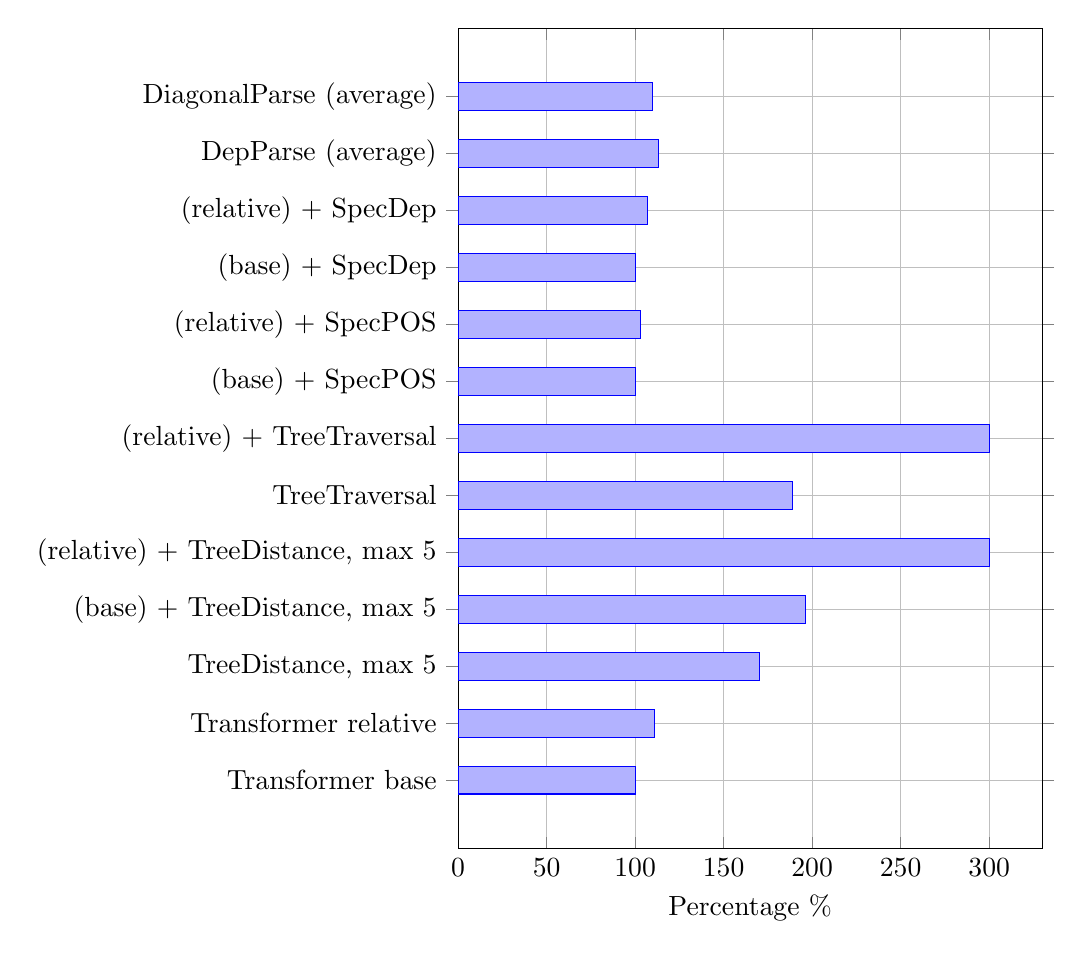
\begin{tikzpicture}
        \begin{axis}[
        height=12cm, width=9cm, grid=major,
        xbar, xmin=0,
        xlabel={Percentage \%},
        symbolic y coords={
            {Transformer base},
            {Transformer relative},
            {TreeDistance, max 5},
            {(base) + TreeDistance, max 5},
            {(relative) + TreeDistance, max 5},
            {TreeTraversal},
            {(relative) + TreeTraversal},
            {(base) + SpecPOS},
            {(relative) + SpecPOS},
            {(base) + SpecDep},
            {(relative) + SpecDep},
            {DepParse (average)},
            {DiagonalParse (average)}
        },
        ytick=data,
        % nodes near coords, nodes near coords align={horizontal},
        ytick=data,
        ]
        \addplot coordinates {
            (100,{Transformer base})
            (111,{Transformer relative})
            (170,{TreeDistance, max 5})
            (196,{(base) + TreeDistance, max 5})
            (300,{(relative) + TreeDistance, max 5})
            (189,{TreeTraversal})
            (300,{(relative) + TreeTraversal})
            (100,{(base) + SpecPOS})
            (103,{(relative) + SpecPOS})
            (100,{(base) + SpecDep})
            (107,{(relative) + SpecDep})
            (113,{DepParse (average)})
            (110,{DiagonalParse (average)})
        };
        \end{axis}
    \end{tikzpicture}
    \caption{Training time to reach 250000 steps on a single GPU nVidia GTX 1080Ti (relative to the \transformerbase).}
    \label{fig:training-speed}
\end{figure}

Having proven that the \transformer NMT model has already captured the dependency syntax, our joint models derived from the \transformer were trained in a comparable time with the single-task \transformerbase.

Training time (including internal evaluation each 1000 steps) to reach 250,000 steps for the \transformerbase is 1 days, 3 hours, 48 minutes on a single GPU nVidia GTX 1080Ti.
On average, our joint dependency parsing and translation model \DepParse took only 13\% longer than the \transformerbase with significant improvement in translation task. \cref{fig:training-speed} also reveals the same for joint diagonal parsing and translation model \DiagonalParse, which took 10\% more time to train.

The encoder's enriched models with specialized attention heads are nearly identical to \transformerbase and \transformerrel.
The \SpecPOS models derived from \transformerbase and from \transformerrel took no extra time comparing to those baselines.
This is also applied to the \SpecDep models. 
However, they are different from the \SpecPOS models that they brought considerable improvements.

While having achieved similar results in translation task, the other set of methods enriching the encoder consumed more time to train.
In detail, the \TreeDistance with maximum distance of 5 consumed 70\% more of the time needed to train \transformerbase, while \TreeTraversal required 89\% more.
When combining with the positional encoding, the \TreeDistance, max 5 took 96\% more to train, but this cost brought significant improvement over both \transformerbase and \transformerrel.
Finally, the total training time for the \TreeDistance, max 5 and the \TreeTraversal when being combined with the relative position are 300\% of the \transformerbase's training time (+200\%). This huge amount of surplus training time were shown to yield improvements as well (\cref{result-enriching}).

The extra amount of training time required by the family of \TreeDistance and \TreeTraversal models were caused by the tree distance and tree encoding matrix's generation, and also the multiplication of these matrices with the key and query vectors.
These computations are quadratic in the length of the input sentence and need to be done on every attention layers of the encoder.
Interestingly, the joint models consumed only a little more time than \transformerbase but brought improvements on translation tasks and good parsing accuracy.
This result was obtained by the fact that our joint models do not add a separate parser on top of the encoder as the common practice in multi-task models, but use the self-attention matrix as the near output layer, then top it with an $argmax$ layer for the head selection.
